\section{EXECUTIVE SUMMARY} 
xxxxxxxxxxxxxxxxxxxxxxxxx

\newpage
\section{INTRODUCTION AND BACKGROUND} 

First Light Fusion (FLF) inertial confinement fusion device is based on the nuclear reaction induced by the impact of a high-speed projectile onto a target mainly made of the fusion fuel (D-T). The use of Liquid Lithium (LL) in form of jet array in the Reactor Chamber (RC) plays a key role as tritium breeder, primary carrier of energy throughout the system, heat and nuclear shielding. \\

\noindent Taking into account that the primary carrier of energy is the LL, its circulation through the system is key to achieve the desired power cycle. This involves ensuring optimal circulation within the primary loop to maximize desired outcomes, such as purification of liquid metal from impurities introduced during operation and efficient management of tritium generated by neutron interactions for overall fuel cycle efficiency.\\

\noindent Considering the requirement to achieve an impurities control in the LL loop of the RC system, the current project studies the feasibility to separate the solid impurities from the liquid metal by means of centrifugal technologies. The first deliverable ref. \cite{SoA} explored the different technologies that potentially could address the LL loop purification.\\

\noindent The objective of the present document is to study from chemical point of view the feasibility of separate the solids impurities from the liquid media (LL), by means of Classical Nucleation Theory (CNT) where fundamental parameters such as critical radius, and its evolution by means of nucleation in the media.

\newpage
\section{SCOPE}\label{sec:scope}
The present document is part of three deliverables: the first deliverable ref. \cite{SoA} addressed the SoA of centrifugal technologies. The second deliverable (which is the current document) is focused in the chemical analysis of the impurities and the technology selection for the centrifuge device, being more specific:

\begin{itemize}
	% ---------------------------------------------------------------------------------------
	\item \textbf{Impurity and Corrosion Analysis:}
	\begin{itemize}
		\item Impurities matrix, given different source. 
		\item Corrosion products identification. 
		\item Maroni's process analysis.
	\end{itemize}
	% ---------------------------------------------------------------------------------------
	\item \textbf{Chemical analysis:}
	\begin{itemize}
		\item Particle Size Distribution (PSD) by means of CNT, for the given FLF impurities: 
		\begin{itemize}
			\item Fe
			\item Cr
			\item AlN
			\item Li2O
			\item LiQ
			\item Li2C2
		\end{itemize}
		\item Impurity critical radius time-evolution: Nucleation analysis.
		\item Homogeneous precipitation: advective-reacting diffusion equation.
	\end{itemize}
	% ---------------------------------------------------------------------------------------	
	\item \textbf{Centrifugal technology selection:}
	\begin{itemize}
		\item Single step separation stage approach.
		\item Multi-step separation stage approach.
		\item Conceptual design approach.
		\item Thermo-hydraulic analytical model.
	\end{itemize}
	% ---------------------------------------------------------------------------------------
\end{itemize}
\subsection{Exceptions} 
N/A
\subsection{Exclusions} 
N/A
\newpage
\section{STRUCTURE OF THE DOCUMENT} % ··························································

The present document it is divided in three main blocks, as per the scope section \ref{sec:scope} list. The blocks are divided by disciplines: impurities analysis SoA, chemical assessment, and engineering assessment including the thermo-hydraulic solid separator mathematical model. \\

\noindent Section \ref{sec:impurity} reviews the impurities and corrosion products in the FLF primary loop. The source of impurities are analyzed from chemical perspective in order to establish a baseline for future analysis. At the same time, a subsection is dedicated to review in the literature the corrosion products from the interaction of liquid lithium with the pipelines made SS316-Ti. The last subsection discusses the Maroni method for tritium extraction and addresses its advantages/disadvantages. \\

\noindent Section \ref{sec:chem} is deeply dedicated to the chemical analysis of the impurities, specially focused on six impurities (established by FLF: Fe, Cr, AlN, Li2O, LiQ, Li2C2) studying the Particle Size Distribution and its temporal evolution to establish the critical radius of the impurities. A specific analysis has been carried to explain the solvers and convergence benchmarks for the Ordinary Differential Equations (ODE's) system develop to understand the different phenomena. Finally, for the non-metallic impurities, a dedicated analysis is the precipitation of those impurities by means of advective-reacting diffusion equation model.  \\

\noindent Section \ref{sec:eng} studies the single and multi-step solid separators with the aim to select the most appropriate centrifugal system for the FLF purification process for the primary loop. Mathematical model has been developed of a solid separator to study different parameter in order to set the possible efficiencies of the device per particle size. Finally, the section describes which device should be studied in the next stage of the current project, from a design and CFD point of view. 

\newpage
\section{METHODOLOGY} % ··························································

The development of the present document follows a methodology (figure \ref{methodology}) based on three lines of work by discipline (SoA, Chemistry, ) that run by batches (presented in box form and sub-tasks). Besides the tasks runs in paralles, they are transversal to all disciplines in terms of technical results, as per the interaction of the outputs and intermediate results. \\

\noindent The figure \ref{methodology} presents the diagram of the methodology and the expected outputs per batch \& disciplines.


\begin{figure}[H]
	\centering
	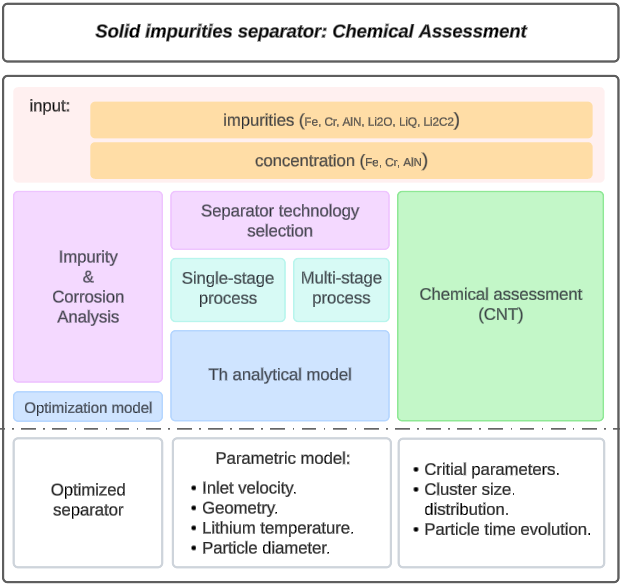
\includegraphics[width=0.8\linewidth]{methodology.png}
	\captionsetup{font=bf, size=small}
	\caption{Methodology}
	\label{methodology}
\end{figure}



\newpage
\section{INPUTS} % ··························································
 To accurately analyze the impact of the impurities from chemical point of view, the following assumptions based on FLF inputhas been considered to target the impurities concentration, as follows:

\begin{tcolorbox}[colback=blue!5!white,colframe=blue!75!black,title=Inputs \& Assumptions]
	The metallic impurities are calculated in the following manner:
	\begin{itemize}
		\item \textbf{135.000 kg/yr} of insoluble metal per year are generated as impurity.
		\item \textbf{8000 hr/yr} of Reactor Chamber (RC) operation.
		\item Assumed concentration:
		\begin{itemize}
			\item 80\% Fe
			\item 10\% Cr
			\item 10\% AlN 
		\end{itemize}
		\item \textbf{1/10 Hz} of Pulsed operation.
		\item \textbf{439.38 Tn} of LL in the loop.
	\end{itemize}
	Impurities mass  produced in 1 pulse in the entire LL loop: \textbf{0.421 Kg}\\
	\underline{Where the concentrations are:}
	\begin{itemize}
		\item Fe $=$ 0.00839 $\text{mol}/m^3$
		\item Cr $=$ 0.00112 $\text{mol}/m^3$
		\item AlN $=$ 0.00142 $\text{mol}/m^3$
	\end{itemize}
	\underline{With an impurities ratio:}
	\begin{itemize}
		\item Li $=$  0.999 e-00
		\item Fe $=$ 1.201 e-07
		\item Cr $=$ 1.613 e-08
		\item AlN $=$ 2.046 e-08
	\end{itemize}
\end{tcolorbox}



\newpage
\section{IMPURITY AND CORROSION ANALYSIS} \label{sec:impurity}% ··························································
\subsection{Impurities Matrix}

Within the scope of the current document, the identification of the impurities source and its main properties is key to provide the necessary context for the coming sections. Given the FLF machines and components, such as: machine gun (upper launcher), Reactor Chamber (RC), and the liquid lithium primary loop, the identified impurity sources are:

\begin{itemize}
	\item \textbf{Lithium initial impurities}.
	\item \textbf{Corrosion:} mainly given by the primary loop (piping and components) made of SS316-Ti, it is assumed at some point the RC vessel made of P91 will be a secondary source of corrosion impurities. The section \ref{sec:corrosion} is dedicated to identify the corrosion products, mechanisms, and its source.
	\item \textbf{Pulsed shot (projectile + target):} considering the input metallic impurities given by FLF (Fe, Cr, AlN), it is assumed in the current document that part of these impurities will be generated at the pulsed operation due to the projectile impact with the target, example of this is the presence of Cr. Future studies will be necessary to identify and classify the impurities result of the pulsed operation. 
\end{itemize}

\subsubsection{Lithium initial impurities}

The initial lithium impurities is a key source in terms of traceability, even more  considering that these impurities can mutate within the system under neutronic irradiation. The Figure \ref{Li_init_imp_chart} shows the list of impurities, ranked in the horizontal axis by concentration and vertically the density of element.  

\begin{figure}[H]
	\centering
	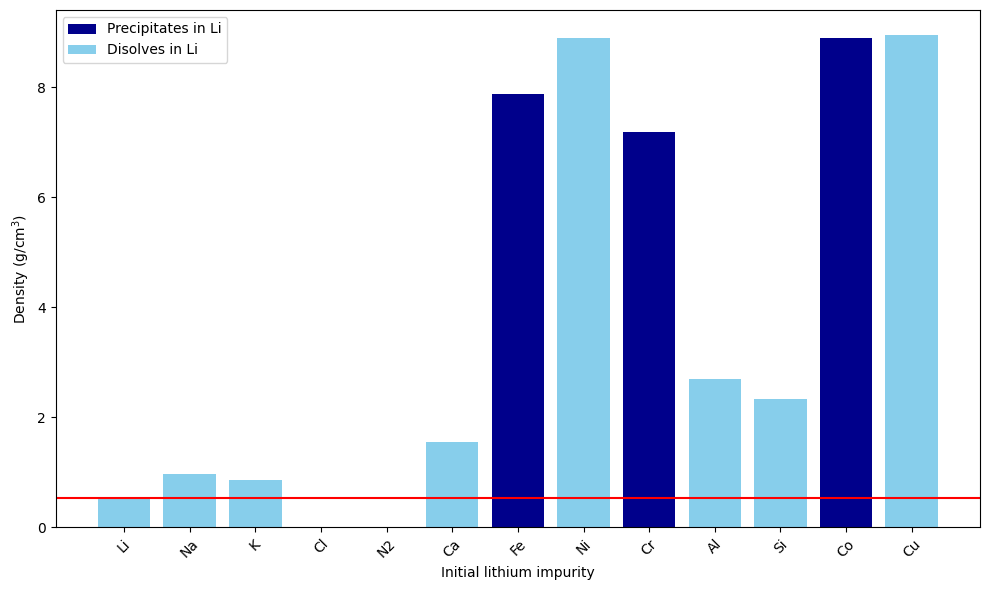
\includegraphics[width=0.97\linewidth]{Li_init_imp_chart.png}
	\captionsetup{font=bf, size=small}
	\caption{Initial lithium impurities.}
	\label{Li_init_imp_chart}
\end{figure}


xxxxxxxxxxxxxxxxxxxxxxxxxxxxxxxxxxxx  explanation here about the results in the graph, 




\begin{table}[H]
	\centering
	\begin{tabular}{ccc}
		\rule[-0.3cm]{0pt}{0.8cm}\textbf{Element}   & \textbf{Content} & \textbf{Density} \\ \Xhline{1.3pt}
		\rule[-0.3cm]{0pt}{0.8cm} Li & 99.98 \% & 0.534 g/cm$^3$ \\ \hline
		\rule[-0.3cm]{0pt}{0.8cm} Na & 0.0034 \% & 0.971 g/cm$^3$ \\ \hline
		\rule[-0.3cm]{0pt}{0.8cm} K & 0.0032 \%  & 0.862 g/cm$^3$ \\ \hline
		\rule[-0.3cm]{0pt}{0.8cm} Cl & 0.0031 \% & 0.003214 g/cm$^3$  \\ \hline
		\rule[-0.3cm]{0pt}{0.8cm} $N_2$ & 0.0020 \% & 0.001250 g/cm$^3$ \\ \hline
		\rule[-0.3cm]{0pt}{0.8cm} Ca & $<$ 0.001 \%  & 1.550 g/cm$^3$ \\ \hline
		\rule[-0.3cm]{0pt}{0.8cm} Fe & $<$ 0.001 \%  & 7.874 g/cm$^3$ \\ \hline
		\rule[-0.3cm]{0pt}{0.8cm} Ni & $<$ 0.001 \%  & 8.900 g/cm$^3$ \\ \hline
		\rule[-0.3cm]{0pt}{0.8cm} Cr & $<$ 0.001 \%  & 7.190 g/cm$^3$ \\ \hline
		\rule[-0.3cm]{0pt}{0.8cm} Al & $<$ 0.001 \%  & 2.702 g/cm$^3$ \\ \hline
		\rule[-0.3cm]{0pt}{0.8cm} Si & $<$ 0.001 \%  & 2.330 g/cm$^3$  \\ \hline
		\rule[-0.3cm]{0pt}{0.8cm} Co & $<$ 0.001 \%  & 8.900 g/cm$^3$ \\ \hline
		\rule[-0.3cm]{0pt}{0.8cm} Cu & $<$ 0.001 \% &  8.960 g/cm$^3$ \\ \hline
	\end{tabular}
	\captionsetup{font=bf, size=small}
	\caption{Lithium initial impurities concentration ref. \cite{Ott1970}.}
	\label{li_imp}
\end{table}








\newpage
\subsection{Corrosion Products}\label{sec:corrosion}
The deliverable \cite{SoA}, listed the lithium impurities and how they are related with the corrosion products together with the effects in steel pipework (SS316). The current section, aims to provide more information gathered form the literature, producing the following table:

\begin{table}[h!]
	%\centering
	\begin{tabular}{p{2cm}p{3cm}p{3.5cm}p{3.5cm}p{2cm}}
		\rule[-0.3cm]{0pt}{0.8cm} \textbf{Li impurities} & \textbf{Effect on Materials} & \textbf{Corrosion Product} & \textbf{Conditions/Notes} & \textbf{References} \\ \hline
		\rule[-0.3cm]{0pt}{0.8cm} Nitrogen & General dissolution and intergranular penetration in stainless steel. & Primary attack via chromium forming Li9CrN5 and iron forming Li3FeN2. & High nitrogen levels lead to corrosion at temperatures between 400-600°C. & \cite{Keough1985}, \cite{Chopra1988}, \cite{Muroga2008}, \cite{Heinzel2006} \\ \hline
		\rule[-0.3cm]{0pt}{0.8cm} Oxygen & Formation and dissolution of unstable ternary oxides. & Li5FeO4, LiCrO2, Li2Ni8O17 formed between Li2O and steels. & Limited information, reactions involve Li2O interacting with Fe, Cr & \cite{IAEA2020}, \cite{Finn1981}, \cite{PULHAM1984} \\ \hline
		\rule[-0.3cm]{0pt}{0.8cm} Carbon & Formation of Cr23C6 precipitates on stainless steel surfaces. & Cr23C6 precipitates enhance chromium concentration at the surface. & Higher weight loss in type 316 stainless steel compared to 9Cr1Mo ferritic steel. & \cite{Parida2019} \\ \hline
		\rule[-0.3cm]{0pt}{0.8cm} Hydrogen & Significant decarburisation of stainless steel. Formation of new phase $Fe_{50}Cr_{43}Mo_{3}Ni_{4}$ on steel surface exposed at 700 $^\circ$C showing intergranular corrosion. & Decrease in carbon content more pronounced in austenitic steel. & Affects both austenitic and ferritic/martensitic steels. & \cite{Parida2019} \cite{Xia2019} \\ \hline
		\rule[-0.3cm]{0pt}{0.8cm} Aluminium & Not known to cause corrosion in stainless steel directly. & Addition of Al reduces weight loss in stainless steel; may form AlN in presence of dissolved nitrogen. & Adding 5wt\% Al to lithium reduced weight loss of type 316 stainless steel. & \cite{Tortorelli1980}, \cite{Keough1985} \\ \hline
		\rule[-0.3cm]{0pt}{0.8cm} No impurities added. & The austenitic area in the welded joint showed morphological changes induced by the dissolution of Ni in Li. The ferritic parts exhibit a fine-grained surface structure. & $M_{23}C_{6}$ and $NiC_x$ particles in sizes of 1-2 $\mu$m. & Study of welded joints (SS316 and SS410) in liquid lithium. & \cite{Xia2019}, \cite{Tsisar2019} \\ \hline
		
	\end{tabular}
	\captionsetup{font=bf, size=small}
	\caption{Corrosion Effects of Impurities in Liquid Lithium on Materials.}
	\label{corrosion_effects}
\end{table}


\newpage
\subsection{Maroni's Process}

The Maroni process has been studied in the SoA deliverable ref. \cite{SoA}, where the process diagram Figure \ref{maroni} of a molten-salt extraction and its stages were analyzed. Nevertheless, the current section is focused in study the advantages/disadvantages of Maroni process, presented in Table \ref{ad_dis_maroni}.  

\begin{figure}[H]
	\centering
	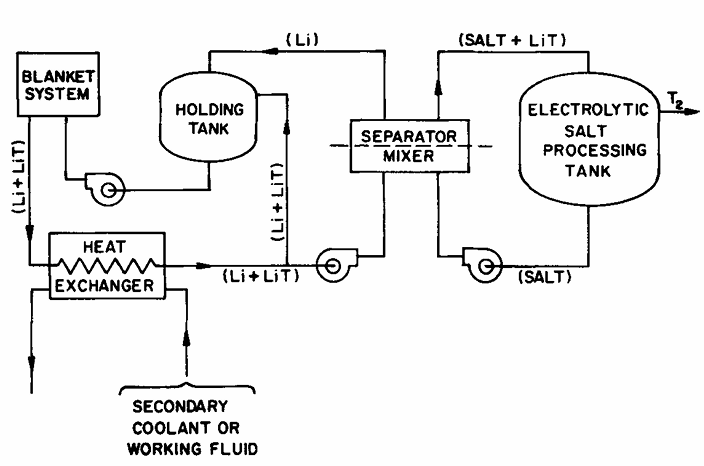
\includegraphics[width=0.7\linewidth]{maroni_schema.png}
	\captionsetup{font=bf, size=small}
	\caption{Schematic diagram of a molten-salt extraction diagram \cite{Maroni1975}.}
	\label{maroni}
\end{figure}

\noindent Before jumping in the Table \ref{ad_dis_maroni}, it is important to remind the Maroni process: based on high temperature molten mixed alkali-metals halide salts (LiCl-KCl at 530 $^\circ$C) as an extraction solvent for the Li + LiT.


\begin{longtable}{p{7.5cm}p{7.5cm}}  
	\rule[-0.3cm]{0pt}{0.8cm} \textbf{Advantages} & \textbf{Disadvantages} \\
	\hline
	\endfirsthead
	
	\rule[-0.3cm]{0pt}{0.8cm} \textbf{Advantages} & \textbf{Disadvantages} \\
	\hline
	\endhead
	
	\endlastfoot
	
	\rule[-0.3cm]{0pt}{0.8cm} \noindent \textbf{Continuous tritium extraction:} The capability to maintain a steady-state tritium inventory within the lithium loop has been incorporated as a critical consideration in the design of the RTPR. This aspect of the design underscores the importance of ensuring a consistent tritium flow and concentration within the system, which is fundamental to the reactor's operational efficiency and safety.  & \textbf{Solubility:} At the operational temperatures of mixing/separating the lithium and salts, the saturation solubility will be reached in the other. The main concern is the presence of salt dissolved in lithium, being significant in terms of corrosion and the products formed under neutronic irradiation (with regard of long-lived radioactive-isotope from the presence of KCl in the lithium jets).  \\
	\hline
	
	
	\rule[-0.3cm]{0pt}{0.8cm} \textbf{Tritium-salts affinity:} The distribution coefficients for 500-600 $^\circ$C are 2.6 for volumetric distribution and 5.8 for molar distribution, being the ratio of tritium content in the salt ($T_{salt}$) to tritium content in lithium ($T_{Li}$) demonstrating that distributions of LiT between the salt and metal phases can be achieved. This advantage of tritium-salts affinity, might allow tritium recovery in the HEX system. & \textbf{Required potential (V):} The extraction of tritium from the salt medium is proposed to be conducted via electrolysis at a potential of 1.5V. However, this process is constrained by the limitation that salt decomposition occurs at potentials exceeding 2.0V. Consequently, to maintain the integrity of the salt medium while ensuring a steady-state tritium inventory, the efficiency of the tritium recovery process must be optimized for operation at the designated 1.5V potential.  \\ \hline
	
	\rule[-0.3cm]{0pt}{0.8cm} \textbf{Density:} Lithium density is less dense than the molten salt by a factor or 3, thus leading to exploit separation system from gravitational settling to centrifugal action. The later separation system could be exploited with hydrocyclones due to its efficiency and low energy cost. & \textbf{Corrosion:} The interaction of materials with lithium, particularly in contexts requiring controlled corrosion rates, remains a significant area of ongoing research. This challenge is further intense in scenarios involving lithium-salt mixtures within mixing/separator devices. To mitigate these issues, the employment of specialized alloys, such as Niobium, was studied in the literature. However, the selection of appropriate materials for lithium loops presents complex considerations, notably due to the specific corrosion behaviors and operational temperature demands associated with fusion nuclear environments. \\ \hline
	
	\rule[-0.3cm]{0pt}{0.8cm}  & \textbf{Volatile elements:} The use of electrolytic process to extract the tritium from salts could involve potential volatile elements such as hydrogen chloride, hydrogen fluoride, hydrogen bromide or its tritium analogs have a direct impact in the feasibility of the tritium extraction in form of gas. Recent studies mitigate the volatile using benign lithium hydroxide (LiOH) or lithium carbonate (Li$_2$CO$_3$).  \\ \hline
	\captionsetup{font=bf, size=small}
	\caption{Maroni process: advantages/disadvantages \cite{Maroni1975}, \cite{Bandhauer2013}.}
	\label{ad_dis_maroni}
\end{longtable}

\newpage
\section{CHEMICAL ANALYSIS} \label{sec:chem}% ··························································
xxxxxxxxxxxxxxxxxxxxxxxxxxxxxxxxx \\
xxxxxxxxxxxxxxxxxxxxxxxxxxxxxxxxx 


\subsection{Particle Size Distribution}
xxxxxxxxxxxxxxxxxxxxxxxxxxxxxxxxx \\
xxxxxxxxxxxxxxxxxxxxxxxxxxxxxxxxx 

\subsection{Temporal Dynamics of Particles Formation}
xxxxxxxxxxxxxxxxxxxxxxxxxxxxxxxxx \\
xxxxxxxxxxxxxxxxxxxxxxxxxxxxxxxxx 

\subsection{Homogeneous Precipitation}
xxxxxxxxxxxxxxxxxxxxxxxxxxxxxxxxx \\
xxxxxxxxxxxxxxxxxxxxxxxxxxxxxxxxx 

\newpage

\section{CENTRIFUGAL TECHNOLOGY SELECTION} \label{sec:eng}% ··························································
With the aim to review the available commercial centrifuges, the current section analyses its application for the purification loop of the RC. \\

\noindent The baseline for the given technologies in sections \ref{sec:sss} and \ref{sec:mss} is taken from the SoA report \cite{SoA}, where centrifuge devices for liquid-liquid and liquid-solid separators has been analyzed. 

\subsection{Single Step Separation Approach}\label{sec:sss}
The aim of this study is to provide the centrifuge technology/ies for FLF primary loop with the purpose to extract the solid impurities in the system. The captured requirements for the impurity loop of FLF has been identified as follows:

\begin{itemize}
	\item Continuous solid impurity extraction.
	\item Material compatibility.
	\item Energy efficiency.
	\item Efficiency for given particle size. 
	\item Operating temperature.
	\item Maintenance and cleaning.
	\item Scalability: maximum flow rate.
	\item Scalability: pressure drop.
	\item Concentration of impurities. 
	\item Residence time.
\end{itemize}

\begin{tcolorbox}[colback=gray!5!white,colframe=gray!75!black,title=Disclaimer]
	The requirements outlined herein pertain specifically to centrifuge technologies and serve as the foundational basis for the current project. Please note that these requirements are not exhaustive and may be subject to expansion or modification as the project progresses through subsequent stages. 
\end{tcolorbox}

\noindent The technologies can be compared based in the criteria given by the requirements, in order to capture which device or set of devices meet successfully the limited framework. Figure \ref{rad_chart} shows a radar chart with the aim to provide a benchmark based on 8 criteria aligned with the solid separator baseline.  

\begin{figure}[H]
	\centering
	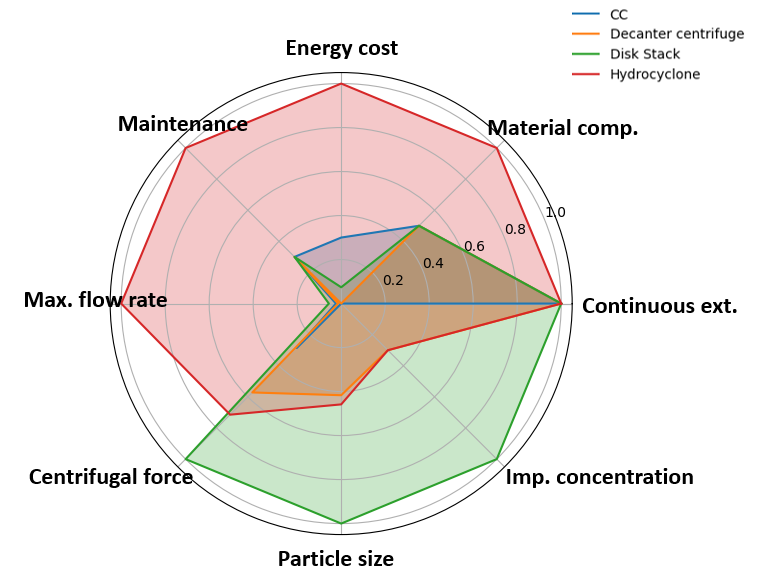
\includegraphics[width=0.85\linewidth]{rad_chart.png}
	\captionsetup{font=bf, size=small}
	\caption{Centrifugal technologies comparison chart}
	\label{rad_chart}
\end{figure}
\begin{figure}[H]
	\centering
	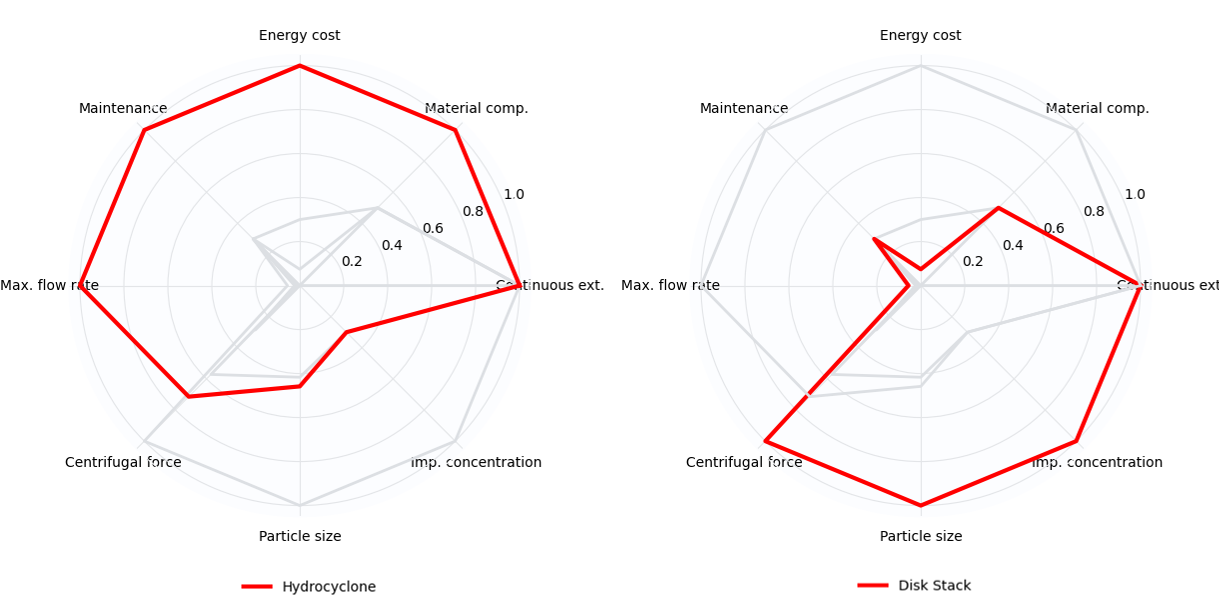
\includegraphics[width=1\linewidth]{rad_chart_comp.png}
	\captionsetup{font=bf, size=small}
	\caption{Hydrocyclone vs Disk Stack separator: radar plot results}
	\label{rad_chart_comp}
\end{figure}

\noindent Figure \ref{rad_chart} shows the performance of 4 centrifugal technologies, with a direct comparison for 8 scores (table \ref{rad_values} has the values used for the comparison, that has been normalized, and inverted for Energy Cost, Particle Size, Imp. Concentration). Hydrocyclone and Disk Stack Separator are the technologies with better performance in the evaluated fields, better single definition can be found in figure \ref{rad_chart_comp}, where:

 \begin{tcolorbox}[colback=blue!5!white,enhanced,breakable,colframe=blue!75!black,title=Hydrocyclone]
 	
 	\textbf{\textit{Advantages:}}
 	\begin{itemize}
 		\item Material compatibility: The hydrocyclone can be constructed using stainless steel, with SS16 being a commercially available option. Additionally, it can be fabricated from Fiber Reinforced Polymers (FRP), offering notable advantages in aggressive environments such as those found in chemical and nuclear applications with activating products. This versatility in material selection ensures adaptability to varying operational requirements and environmental conditions, enhancing the hydrocyclone's reliability and longevity in demanding settings.
 		\item Maintenance: Characterized by its absence of rotatory components, comprising four conical segments interconnected via flange bolted connections. This design feature ensures facilitated access to the internal cavity, enabling procedures for cleaning, replacement, or repair purposes.
 		\item Energy cost: The inherent design features, including a tangent inlet inducing a vortex through the cone, eliminates the necessity for moving parts, thus precluding the need for an engine. This architectural advantage translates into significant energy savings, as the hydrocyclone operates without any associated energy costs. Moreover, rigorous examination of inlet velocity's impact underscores the meticulous engineering approach applied to optimize performance.
 		\item Flow rate: It demonstrates superior flow rate management in comparison to the other three analyzed technologies. Moreover, it is commercially available to operate within a manifold architecture, allowing for efficient handling of large volumes. Consequently, it emerges as a prime candidate for processing the primary loop lithium in a single operation.
 	\end{itemize}
 	
 	\textbf{\textit{Disadvantages:}}
 	
 	\begin{itemize}
 		\item Particle size: Commercially available up to a particle size of 12 $\mu m$, with an impressive efficiency rate of 98\%, while maintaining scalability with a compromise on pressure drop (10-200 KPa). This equilibrium represents the optimal trade-off. Consequently, particles below 12 $\mu m$ can be captured by the hydrocyclone; however, ensuring consistent efficiency for particles of this size is not assured. Therefore, additional stages specifically designed for particles of this size range must be incorporated into the purification system to ensure thorough filtration and purification.
 		\item Impurity concentration: The technology's optimal operational range encompasses concentrations of impurities in the medium exceeding 10\%. Therefore, it is recommended to position this technology as the initial stage within the purification system. This strategic placement ensures efficient removal of contaminants at higher concentrations, thereby enhancing the overall effectiveness of the purification process. Future stages may address more accurate the impurity concentration in the system.
 	\end{itemize}
 	
 	\textbf{\textit{Assessment:}} The hydrocyclone offers exceptional material compatibility, maintenance-friendly design (without of rotatory components), with negligible energy costs and superior flow rate management, based on manifold architectures: the hydrocyclone emerges as an ideal candidate for processing the primary loop fluid. Despite limitations in capturing particles below 12 $\mu m$ and optimal operation at impurity concentrations exceeding 10\%, strategic integration within purification systems enhances overall effectiveness.
 	
 \end{tcolorbox}
 \begin{tcolorbox}[colback=blue!5!white,enhanced,breakable,colframe=blue!75!black,title=Disck Stack Separator]
		\textbf{\textit{Advantages:}}
	\begin{itemize}
		\item Particle size: One of the most notable strengths of this technology lies in its ability to effectively capture particles as small as 1 $\mu m$, facilitated by its high centrifugal force and innovative ribs cavity design, which accelerates solid precipitation. Particularly advantageous in scenarios where prior classification or clearance of larger particle sizes has been performed, allowing for optimal exploitation of its particle-capturing capabilities.
		\item Impurity concentration: The operational range for these devices remains optimal when impurity concentrations are below 10\%, presenting an advantageous characteristic when integrated into multi-stage system operations.
		\item Centrifugal force: As a high-speed separator capable of achieving up to 14,000 G, the disk stack separator offers a distinct advantage due to its efficient operation at relatively low energy costs, contrasting with decanter centrifuges. While centrifuge contractor may require similar energy inputs, they do not attain comparable levels of centrifugal force, highlighting the disk stack separator's pivotal role in separation processes based on its design principles.
	\end{itemize}
	
	\textbf{\textit{Disadvantages:}}
	
	\begin{itemize}
		\item Energy cost: Exhibits relatively higher energy consumption compared to alternative solutions. This aspect should be considered in the evaluation of operational costs and efficiency metrics within the full-scale context.
		\item Maintenance: The trade-off associated with attaining high-speed rotation velocities may influence the maintenance of components, wherein direct access to elements is not a direct action, requiring mechanical assembly-disassembly processes that are less straightforward compared to hydrocyclones.
		\item Flow rate: The limited maximum flow rate capacity of such devices makes them unsuitable for fully processing all the lithium within the primary loop. Furthermore, the absence of commercially available manifolds presents a challenge. Therefore, a rigorous study could be needed to strategically place these devices within the system, coupled with the feasibility assessment for developing a manifold configuration to optimize operational efficiency.
	\end{itemize}
	
	\textbf{\textit{Assessment:}} The Disk Stack Separator offers good particle capture capabilities, particularly for particles as small as 1 $\mu m$, making it ideal for scenarios requiring precise filtration after prior particle classification. However, its higher energy consumption and maintenance complexities warrant careful consideration. When compared with hydrocyclones, which excel in energy efficiency and maintenance simplicity, they form complementary components in a comprehensive purification system, each tailored to specific operational requirements and constraints. Integrating both technologies strategically within a multi-stage system can optimize overall efficiency and performance, complementing their disadvantages.
	
	
\end{tcolorbox}
 \begin{tcolorbox}[colback=blue!5!white,enhanced,breakable,colframe=blue!75!black,title=Decanter Centrifuge]
	Decanter centrifuges demonstrate comparable performance to hydrocyclones in particle size handling, centrifugal force generation, and impurity concentration control. However, hydrocyclones offer superior energy efficiency, enhanced material compatibility, and lower maintenance requirements, presenting clear advantages. Notably, hydrocyclones excel in maximizing the maximum flow rate, making them a preferred choice in scenarios prioritizing throughput efficiency and operational cost-effectiveness.
\end{tcolorbox}
 \begin{tcolorbox}[colback=blue!5!white,colframe=blue!75!black,title=Centrifuge Contactor]
	While centrifuge contactors offer the advantage of producing four-phase liquid separation, they do not present a significant advantage in the fields compared to hydrocyclones. The technology lacks suitability in efficiently handling impurities at required flow rates with the precision demonstrated by alternative technologies, diminishing its practical utility in for the primary loop.
\end{tcolorbox}

\newpage
\subsection{Multi-Step Separation Approach}\label{sec:mss}
In the context of a multi-stage separation process, the integration of hydrocyclones and Disk Stack Separators offers a comprehensive solution for fluid purification. The hydrocyclone, as particle cut-off controlled by operation parameters, is particularly adept at classifying and separating coarser particles ($>$ 12 $\mu m$), thereby facilitating the initial removal of larger impurities. Its attributes, including superior material compatibility and a maintenance-friendly design, make it a suitable choice for efficiently processing substantial fluid volumes, thanks to its ability to handle high flow rates and adapt to various manifold configurations.\\


\noindent However, the hydrocyclone's inherent limitations, such as its inability to capture particles below 12 $\mu m$ and its optimal operation in scenarios with impurity concentrations above 10\%, necessitate additional stages for thorough purification. This is where the Disk Stack Separator comes into play, especially in scenarios where specific targets, such as low impurities or activated products separated by density differences like Li-H, need to be addressed. Renowned for its exceptional particle capture efficacy, particularly for particles as small as 1 $\mu m$, the Disk Stack Separator strategically placed downstream of the hydrocyclone enhances the purification process by effectively removing finer particles and residual impurities at low concentrations (up to 0.05\%), thereby ensuring the level of lithium purity.\\


\noindent Despite its advantages, the Disk Stack Separator incurs relatively higher energy consumption and maintenance complexities compared to the hydrocyclone. Therefore, meticulous attention is needed in optimizing the integration of these technologies to ensure overall efficiency. For example, incorporating the Disk Stack Separator as a secondary stage in the purification process allows for precise filtration after larger particles have been removed by the hydrocyclone, as shown in Figure \ref{multi_stage}. At the same time, it raises the requirement to project a future device that captures the high efficiency for small particles at the energy cost and lithium volumes of the hydrcyclone.

\begin{figure}[H]
	\centering
	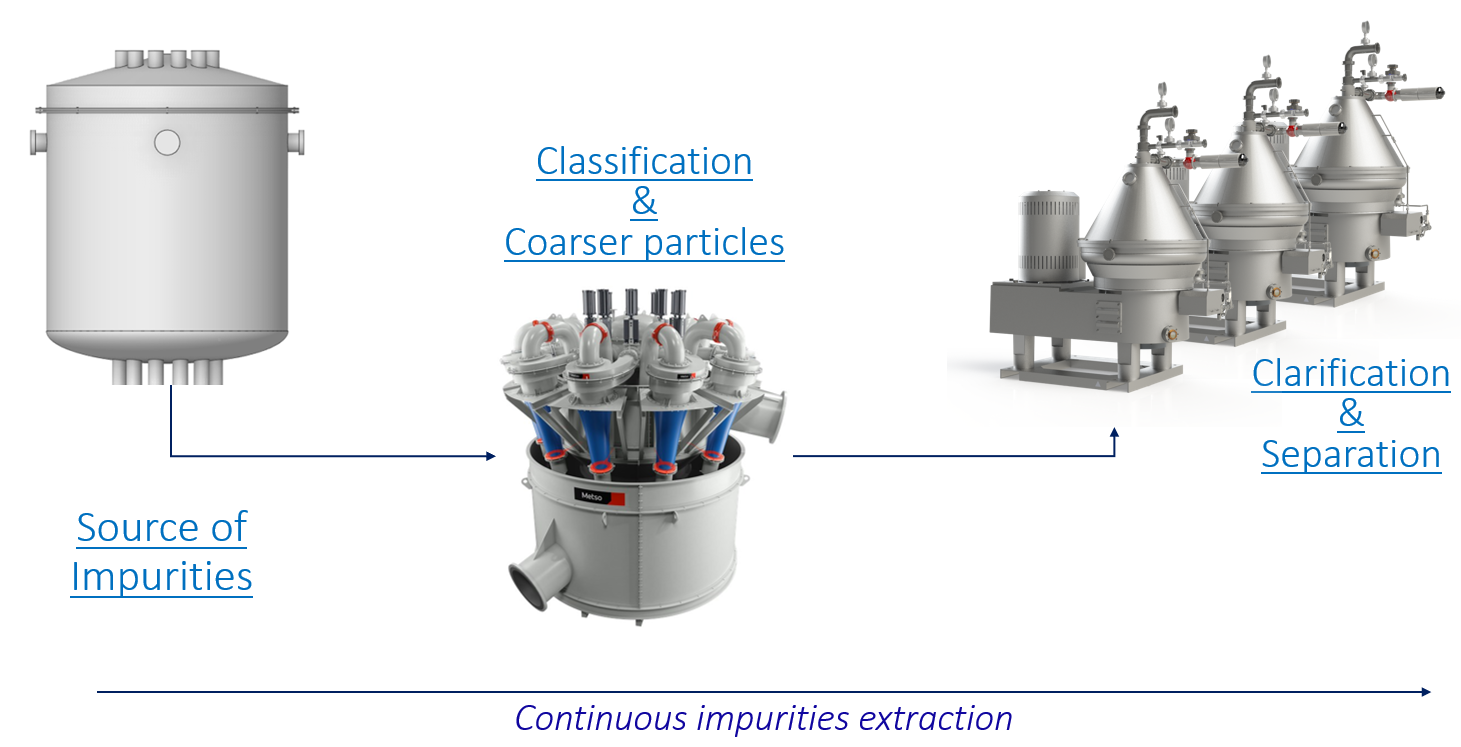
\includegraphics[width=0.9\linewidth]{multi_stage.png}
	\captionsetup{font=bf, size=small}
	\caption{Multi stage configuration}
	\label{multi_stage}
\end{figure}

\noindent In this multi-stage paradigm, the symbiotic relationship between the hydrocyclone and Disk Stack Separator maximizes each technology's strengths while mitigating respective weaknesses. \\

\noindent The relevant technical specifications for both technologies are delineated in Figure \ref{multi_stage_technical}. This technical data serves as the foundational benchmark for subsequent stages of the project, guiding the development of solutions aligned with the current multi-stage framework. The analysis of this data informs decisions regarding the integration of technologies, aiming to optimize the process schema and ultimately enhance overall efficiency and effectiveness.

\begin{figure}[H]
	\centering
	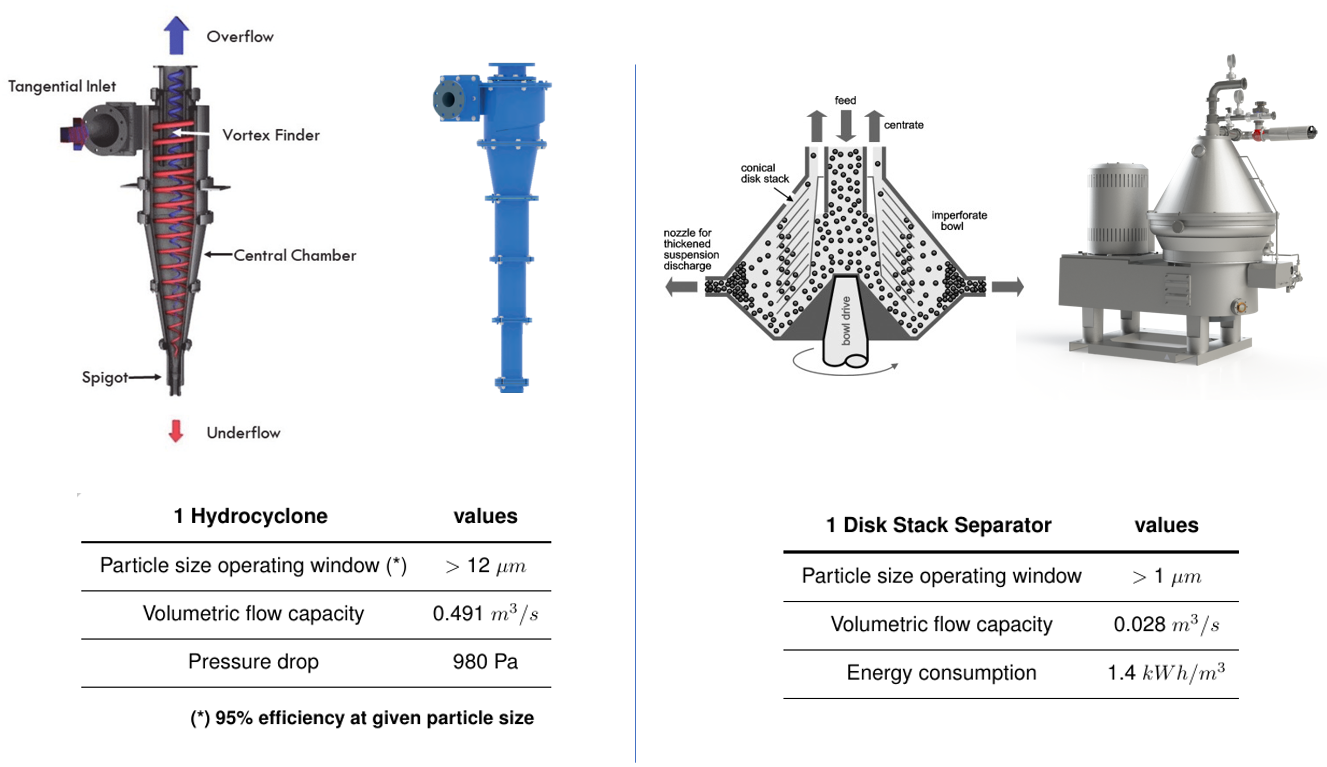
\includegraphics[width=1\linewidth]{multi_stage_technical.png}
	\captionsetup{font=bf, size=small}
	\caption{Multi stage device data-sheet}
	\label{multi_stage_technical}
\end{figure}

\newpage
\subsection{Hydrocyclone: Mathematical modelling}

%\section{Mathematical model}
Cyclone separators are widely used in the field of chemical, mine and petroleum industries. ref.\cite{Concha2007} With the advantages of relative simplicity to fabricate, low cost to operate and good adaptability to extremely harsh conditions, cyclone separators have become one of the most important particle removal devices which are preferably utilized in both environmental and chemical engineering.
In order to describe the performance of cyclone separators, many (gas or liquid)-particle separation theories were developed using different methods with different simplifications and assumptions.
All these can be roughly divided into the pure theory, the semi-empirical theory and the numerical simulation. The former two include the equilibrium-orbit model, time-of-flight model and hybrid model, etc., the later mainly refers to the computation fluid dynamics (CFD) approach ref.\cite{Altmeyer2003}.

In detail, the equilibrium-orbit model, as an early methodology of particle separation, determines the particle size for which centrifugal force is exactly balanced by the drag force. Correspondingly, the collection efficiency for the critically sized particle is often assumed to be 50\% efficiency called cut particle diameter $d_{c,p}$ ref.\cite{Zhao2011}.

 In this section, the necessary parameters and assumptions are defined to correctly define the equilibrium orbit model and obtain an expression for the cyclone separation efficiency.
 \begin{tcolorbox}[colback=blue!5!white,colframe=blue!75!black,title=Assumptions]
The following assumption have been made in order to develop the equilibrium-orbit model ref. \cite{Wei2016}: 
\begin{itemize}
	\item The particle is spherical in shape, the motion of the single particle is not influenced by the presence of neigh-boring particle.
	\item The tangential velocity of the particle is same as the disperse phase stream; and with the particle is the right dispersed phase, the radial velocity direction fo the particle always point to inner vortex.
	\item  The particle move into the inner vortex is the only way to be separated.  
\end{itemize}
\end{tcolorbox}


Figure (\ref{cyclone_schema}) show a generic scheme of the cyclone and the description of the different variables is presented in table (\ref{variable_cyclone_description}).


\begin{figure}[H]
	\begin{minipage}[b]{.4\linewidth}
		\centering
		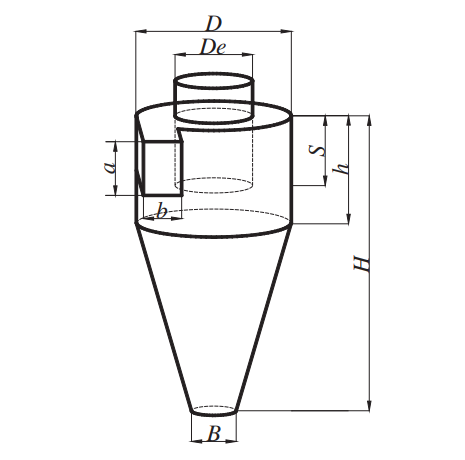
\includegraphics[width=1\linewidth]{images/schema.png}
		\captionsetup{font=bf, size=small}	
		\captionof{figure}{Schematic diagram of typical cyclone dimensions.}
		\label{cyclone_schema}
	\end{minipage}\hfill
	\begin{minipage}[b]{.59\linewidth}
		\centering
	\begin{tabular}{cc}
		\hline
			\rule[-0.3cm]{0pt}{0.8cm}\textbf{variable} & \textbf{description}                                \\ \hline
			\rule[-0.3cm]{0pt}{0.8cm}$a$                 & Cyclone inlet height (m)                            \\ \hline
			\rule[-0.3cm]{0pt}{0.8cm}$b$                 & Cyclone inlet width (m)                             \\ \hline
			\rule[-0.3cm]{0pt}{0.8cm}$B$                 & Particle outlet diameter (m)                        \\ \hline
			\rule[-0.3cm]{0pt}{0.8cm}$D$                 & Cyclone body diameter (m)                           \\ \hline
			\rule[-0.3cm]{0pt}{0.8cm}$D_e$              & Liquid outlet diameter (vortex finder diameter) (m) \\ \hline
			\rule[-0.3cm]{0pt}{0.8cm}$h$                 & Cyclone cylinder height (m)                         \\ \hline
			\rule[-0.3cm]{0pt}{0.8cm}$H$                 & Cyclone height (m)                                  \\ \hline
			\rule[-0.3cm]{0pt}{0.8cm}$S$                 & Liquid outlet duct length (m)                       \\ \hline
	\end{tabular}
		\captionof{table}{Description of the geometrical variables of one cyclone.}
		\label{variable_cyclone_description}
	\end{minipage}
\end{figure}


\subsection{Fluid model}
%For this problem there are 2 types of phenomena present to describe the flow pattern. The first zone is called the forced vortex, which occurs between r=0 and r=b/2 approximately where the tangential velocity is linear with the angular velocity w (v=w r). On the other hand, we have a free vortex given by the equation:

Swirling flow, or vortex flow, occurs in different types of equipment, such as cyclones, hydrocyclones, spray dryers and vortex burners. Two types of ideal swirling flows are ref.\cite{Marthinussen2011}: 
\begin{itemize}
	\item Forced vortex flow: swirling flow with the same tangential velocity distribution as a rotating solid body.
	\begin{equation}
		v_{\theta,f}=\omega r 
	\end{equation}
	\item Free vortex flow: the way a frictionless fluid would swirl. The tangential velocity in such a swirl is such that the moment-of-momentum of fluid elements is the same at all radius. 
	\begin{equation} \label{free_vortex_flow}
		v_{\theta,f}(r)=\frac{\kappa}{r^n} \text{  where } 0.4<n<0.9 
	\end{equation}	
	where $\kappa$ is a geometrical parameter and $n$ is a experimental value taken 0.88 as in ref.\cite{Sabbagh2014} 
\end{itemize} 
Figure (\ref{tangential_velocity}) show the schema of the real tangential velocity distribution and the comparison with the forced and free vortex flow.

\begin{figure}[H]
	\centering
	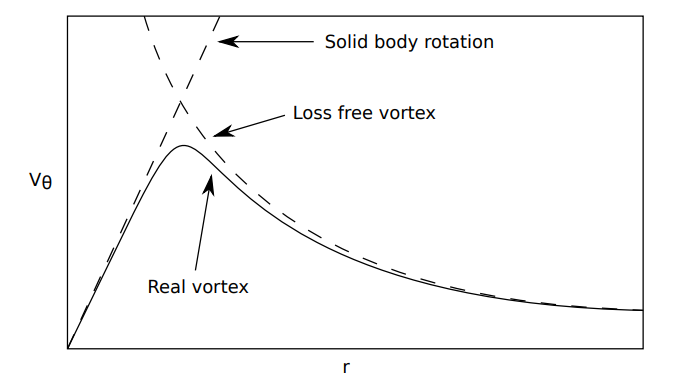
\includegraphics[width=0.5\linewidth]{images/tangential_velocity_schema.png}
	\captionsetup{font=bf, size=small}
	\caption{Scheme of the 2 ideal vortex model and the tangential velocity distribution in a real vortex. ref.\cite{Marthinussen2011}}
	\label{tangential_velocity}
\end{figure}

\subsection{Motion of suspended particles}
In a hydrocyclone, the particles of interest are almost always moving relative to the liquid at their terminal velocity, and the terminal velocity of a given particle determines whether the particle will be captured or lost.

Applying Newton’s law to a particle moving in a fluid, equating its mass times acceleration to the sum of the forces acting on it, gives :
\begin{equation}
	m \frac{d v}{d t}= F_{body} + F_{drag} + F_{unsteady}
\end{equation}
where the body force is normally due to a centrifugal force and the fluid drag represents the drag acting on a
particle that moves with a steady velocity relative to the fluid ref.\cite{Sabbagh2014} .
According to several authors ref.\cite{Concha2007,Marthinussen2011}, it turns out that these unsteady terms can be ignored both for the case of a gas cyclone and a hydrocyclone, as practical plant experience with their design and operation indicates that it is not necessary to include either of the terms.


%\subsubsection*{Centrifugal Force}
The centrifugal force (first term on the right part ) can be expressed as :
\begin{align}
	F_{body}=F_{centrifugal}=V_p \left( \rho_p-\rho_{f} \right) \textbf{a}
\end{align}
where $V_p$ is the particle volume, $\rho_p$ is the particle density, $\rho_f$ is the fluid density and $\textbf{a}$ is the global effect of the radial and angular particle acceleration. 

In cylindrical coordinate, omitting the axial contribution, 
\begin{itemize}
	\item $a_r= \frac{d v_{r,p}}{d t}= \frac{d^2 r}{d t^2 }$ particle radial acceleration 
	
	\item $a_c= r \left( \frac{d \theta}{d t}\right)^2= r \left(\frac{v_{\theta,f} (r)}{r} \right)^2 $ particle angular acceleration
	
\end{itemize}
assuming that the radial particle acceleration in the steady state is negligible, the centrifugal force is equal to:
\begin{equation}
	F_{centrifugal}= \frac{1}{6} \pi d_p ^3 \cdot (\rho_p -\rho_f) \cdot \frac{v_{\theta,f} ^2(r)}{r}
\end{equation}

%\subsubsection*{Drag Force}
on the other hand, when the particle Reynolds number is low ($Re_p = \frac{d_p v_{r,p}}{\nu}<<1$), the
equations of motion for the fluid moving around the particle can be solved, and the drag force 
calculated. If there is no slip between fluid and particle surface, the particle velocity is
equal to the velocity of the fluid at the surface, the result is Stokes drag law: 
\begin{equation}
	F_{drag}=3 \pi  \mu d_p v_{r,p}(r) 
\end{equation}
Therefore, in the steady state, the drag force have to be equal that the centrifugal force:

\begin{equation}
	\sum F_p = 0 \Rightarrow F_{centrifugal}= F_{drag}  
\end{equation}
and the radial velocity of the particle can be expressed as a function of the angular velocity of the fluid given by the vortex flow model as
\begin{equation} \label{radial_velocity_particle}
	v_{r,p}(r)= \frac{\Delta \rho d_p ^2   }{18 \mu } \cdot \frac{v_{\theta,f}^2(r)}{r}
\end{equation}


The following subsections define different parameters necessary to calculate the cyclone separation efficiency.


\subsection{Cyclone effective volume}
To avoid the non-uniform effect on particle collection distance caused by difference between cylindrical and conical shape, the cylinder-conical geometry is equivalently modified as a right cylinder cyclone according to the principle of conservation of effective volume.
The equivalent cyclone volume ($V_{cs}$) and  radius ($R$) can be calculated by: ref.\cite{Zhao2011}
\begin{equation}
	V_{cs}=
	\begin{cases}
		 \frac{\pi D^2 h}{4} +\frac{\pi D^2 }{4} \cdot \frac{S+l-h}{3} \cdot \left[ 1+ \frac{D_c}{D}+ \left(\frac{D_c}{D} \right)^2  \right] ,& \text{if } l\leq (H-S)\\
		\frac{\pi D^2 h}{4} +\frac{\pi D^2 }{4} \cdot \frac{H-h}{3} \cdot \left[ 1+ \frac{B}{D}+ \left(\frac{B}{D} \right)^2  \right],& \text{if } l> (H-S)
	\end{cases}
\end{equation}



\begin{equation} \label{effective_radious_equation}
	{R^*} _w= 
	\begin{cases}
		\left[ \frac{V_{cs}}{\pi (S+l)}\right]^{1/2} ,& \text{if } l\leq (H-S)\\
		\left[ \frac{V_{cs}}{\pi H}\right]^{1/2},& \text{if } l> (H-S)
	\end{cases}
\end{equation}
where $D_c= D - \frac{(D-B)(S+l-h)}{H-h}$ and $l$ is called as the natural vortex length of cyclone separator. It is defined as the vertical distance from the bottom of the vortex finder to the end of the vortex at which the outer vortex is reversed or turned into the inner vortex. $l$ is actually the effective vortex length in cyclone separator if it is less than the dimension $H–S$. Otherwise, $H–S$ should be the effective vortex length because it depends on the geometrical dimensions of cyclone.
The most famous and widely used relation for estimating the natural vortex length is the Alexander’ formula ref.\cite{Zhao2011}: 
\begin{equation}
	l=2.3 \left( \frac{D^2}{a b}\right)^{1/3}
\end{equation}

\subsection{Residence time model} 
The residence time $t_{res}$ is the average time  that a particle is inside the cyclone. The expression to calculate $t_{res}$ depend of the geometry of the cyclone and the inlet volumetric flow rate, so according to the geometry selected (Figure \ref{cyclone_schema}) the residence time can be calculates as ref.\cite{Zhao2011}:
\begin{equation}\label{residence_time_equation}
	t_{res}= 
	\begin{cases}
		\frac{\pi \left( R^2 - R_e ^ 2\right) }{Q/2} \cdot l,& \text{if } l\leq (H-S)\\
		\frac{\pi \left( R^2 - R_e ^ 2\right)}{Q/2} \cdot (H-S),& \text{if } l> (H-S)
	\end{cases}
\end{equation}

\subsection{Separation efficiency model}
In order to calculate the separation efficiency of the cyclone, a balance of mass was made in the volume of control presented in the Figure (\ref{volume_control}) ref.\cite{Zhao2011,Wei2016}.
\begin{figure}[H]
	\centering
	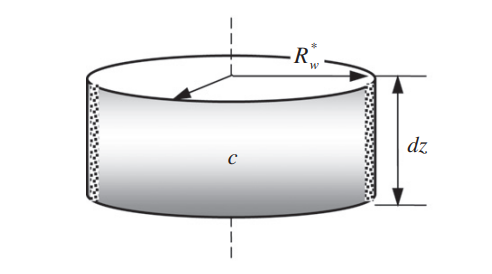
\includegraphics[width=0.5\linewidth]{images/control_volume.png}
	\captionsetup{font=bf, size=small}
	\caption{volume of control used in the separation efficiency model. ref.\cite{Zhao2011}}
	\label{volume_control}
\end{figure}
In this control volume, it is assumed that uncollected particles in any plane perpendicular to the cyclone axis presents a status of complete radial back-mixing, the boundary layer near the equivalent wall is neglected and particles which move to the equivalent wall will be trapped. If the particle concentration in the control volume is
$c$, then the particle flux toward the equivalent wall is $c v_{r,p}({{R^*}} _w)$ . Therefore, over a height $dz$ the sedimentation rate of particles at the equivalent wall is $ 2 \pi {{R^*}} _w c v_{r,p}({R^*} _w) $ . Correspondingly, the rate of particles separated from the control volume is $c \pi {{R^*}} _w^2 dz$.
According to particle mass balance, we have:


\begin{align}
	\frac{d M}{d t }=& \sum M_{in} -\sum M_{out}\\
	\frac{d(c \pi {R^*} _w^2 dz)}{dt}=& -\sum M_{out}= - c v_{r,p}({R^*} _w) 2 \pi {R^*} _w dz\\
	\frac{d c}{d t}=& - \frac{2v_{r,p}(R* _w)}{{R^*} _w} \cdot c \\
	\frac{c(t)}{c_0}=& exp \left(- \frac{2v_{r,p}({R^*} _w) t}{{R^*} _w} \right)
\end{align}

Integrating, with $c(t=0)=c_0$ and $c_{final}=c(t_{res})$ where $t_{res}$ is the particle residence time:

\begin{equation}
	\frac{c_{final}}{c_{0}}= exp \left(- \frac{2v_{r,p}({R^*} _w) t_{res}}{{R^*} _w} \right)
\end{equation}
therefore, the separation efficiency is defined as 
\begin{align} 
	\eta=&1-\frac{c_{final}}{c_{0}}\\
	\eta=&1- exp \left(- \frac{2v_{r,p}({R^*} _w) t_{res}}{{R^*} _w} \right) \label{efficiency_equation}
\end{align}
where $v_{r,p}({R^*} _w)$ is the particle settling velocity at the equivalent wall
and is calculated according to Eq. (\ref{radial_velocity_particle}) 

\section{Results: Parametric analysis}

For the following analysis, the geometric dimensions present in the table \ref{input_information} have been used as a basis. This information was used to see how the separation efficiency of the cyclone varies when the Lithium temperature, the diameter of the cyclone and the inlet flow change. 

\begin{table}[H]
	\centering
	\begin{tabular}{cc}
			\rule[-0.3cm]{0pt}{0.8cm} \textbf{variable} & \textbf{value} \\ \hline
			\rule[-0.3cm]{0pt}{0.8cm}\textbf{$D$}                            & 0.5 m          \\ \hline
			\rule[-0.3cm]{0pt}{0.8cm}\textbf{$\frac{De}{D}$}                        & 0.5            \\ \hline
			\rule[-0.3cm]{0pt}{0.8cm}\textbf{$\frac{a}{D}$}                         & 0.5            \\ \hline
			\rule[-0.3cm]{0pt}{0.8cm}\textbf{$\frac{b}{D}$}                         & 0.2            \\ \hline
			\rule[-0.3cm]{0pt}{0.8cm}\textbf{$\frac{S}{D}$}                         & 0.5            \\ \hline
			\rule[-0.3cm]{0pt}{0.8cm}\textbf{$\frac{H}{D}$}                         & 4              \\ \hline
			\rule[-0.3cm]{0pt}{0.8cm}\textbf{$\frac{h}{D}$}                         & 1.5            \\ \hline
			\rule[-0.3cm]{0pt}{0.8cm}\textbf{$\frac{B}{D}$}                         & 0.375          \\ \hline
			\rule[-0.3cm]{0pt}{0.8cm}\textbf{Fluid material}               & Lithium        \\ \hline
			\rule[-0.3cm]{0pt}{0.8cm}\textbf{Fluid Temperature}            & 688 K          \\ \hline
			\rule[-0.3cm]{0pt}{0.8cm}\textbf{Particle material}            & Fe            \\ \hline
	\end{tabular}
	\caption{Input information used for the parametric analysis section}
	\label{input_information}
\end{table}
\subsection{Parametric analysis: Temperature}
Figure (\ref{temperature_cyclone}) shows the efficiency as a function of the particle diameter of Fe for the temperature of the Start-Up, HEX outlet and lower tank calculated in ref. \cite{power_scenario}. 


\begin{figure}[H]
	\centering
	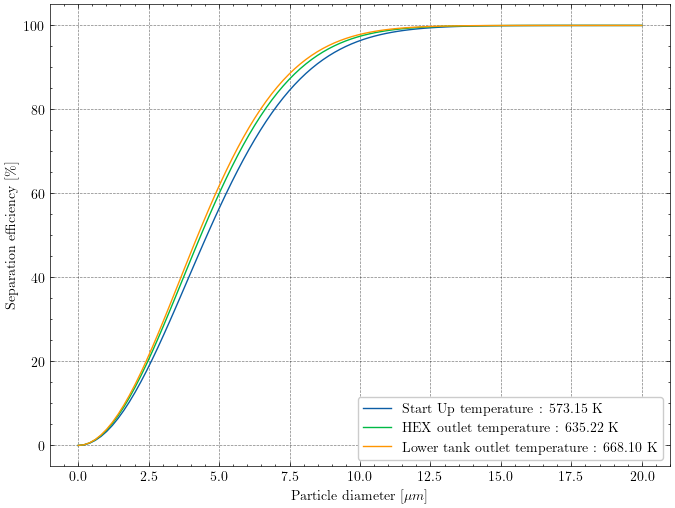
\includegraphics[width=0.5\linewidth]{images/efficiency_vs_Temperature.png}
	\captionsetup{font=bf, size=small}
	\caption{Separation efficiency as a function of the particle diameter of Fe for different temperatures.}
	\label{temperature_cyclone}
\end{figure}
As the temperature increases, the fluid viscosity decreases, so the drag force  decrease and the particle velocity increase. Also, the difference in density fluid-particle also increases (since the density of lithium decreases with temperature) so that the centrifugal force grow. Those effects allows efficiency to increase with temperature.
\subsection{Parametric analysis: Cyclone diameter}
Figure (\ref{cyclone_diameter})  shows the separation efficiency as a function of the particle diameter of Fe for different cyclone diameters.

\begin{figure}[H]
	\centering
	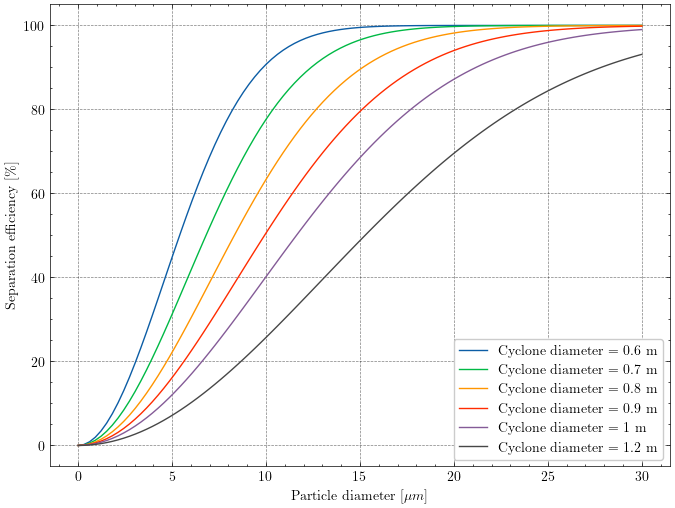
\includegraphics[width=0.5\linewidth]{images/efficiency_vs_cyclone_diameter.png}
	\captionsetup{font=bf, size=small}
	\caption{}
	\label{cyclone_diameter}
\end{figure}
By increasing the diameter and keeping the scaling and flow variables constant, the velocity in the inlet decreases. This decrease causes that the velocity of the particles to drop and the efficiency to drop. On the other hand, as the diameter increases, the residence time increases given by the equation (\ref{residence_time_equation}) and this effect tends to increase efficiency, however, it is not as important as the other effect mentioned before.

%By increasing the diameter,  it is possible to process more flow in each cyclone. However, the separation efficiency decreases. It is a compromise decision since is needed to know the minimum particle diameter that have to be eliminated.
Thus, there is a trade-off in deciding the optimal cyclone diameter, and it will also depend on the minimum particle diameter of the impurities which need to be eliminated.
\subsection{Parametric analysis: volumetric inlet flow rate}
Given one of the limitations of cyclones is the possibility of scaling efficiency to industrial-type flows, in the chemical or mine industry it is very common to use more than 1 cyclone in parallel ref. \cite{Concha2007}. For this reason it is of interest to know how the efficiency changes as we increase the volumetric inlet flow rate of the cyclone.

Figure (\ref{inlet_VRF}) show the separation efficiency as a function of the particle diameter for different volumetric inlet flow rate form from 0.5 to 3.5 $m^3/s$ (similar to pilot plant). 

\begin{figure}[H]
	\centering
	\begin{subfigure}{.49\textwidth}
		\centering
		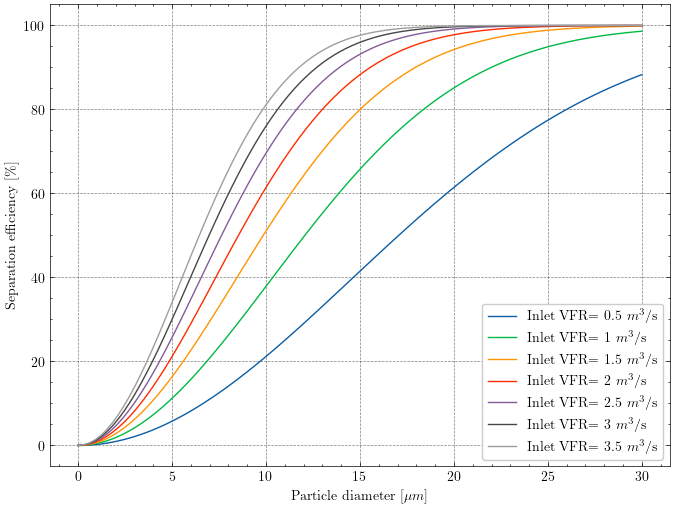
\includegraphics[width=1.0\linewidth]{images/efficiency_vs_inlet_VFR.png}
		\caption{}
		\label{inlet_VRF}
	\end{subfigure}
	\begin{subfigure}{.49\textwidth}
		\centering
		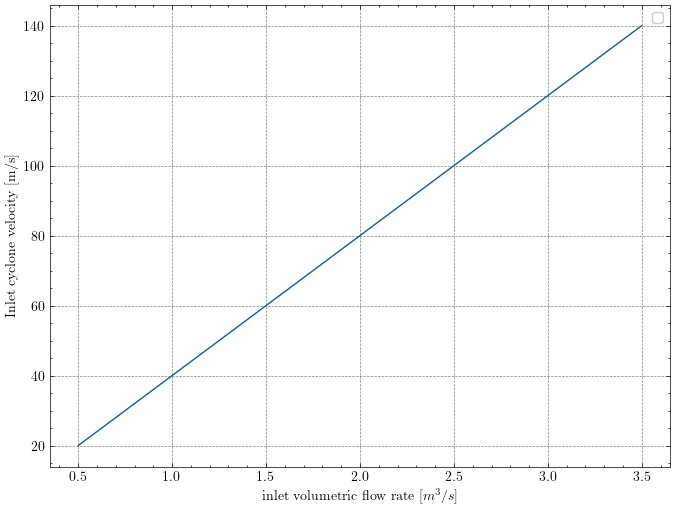
\includegraphics[width=1.0\linewidth]{images/inlet_VRF_vs_inlet_velocity.png}
		\caption{}
		\label{inlet_velocity}
	\end{subfigure}
	\captionsetup{font=bf, size=small}
	\caption{ }
	\label{}
\end{figure}

It can be seen that as volumetric flow rate decrease, the separation efficiency decreases. This is because as the flow rate at the inlet of the cyclone decreases, the velocity in the inlet drop (Figure \ref{inlet_velocity}) and consequently the velocity with which the particle heads towards the walls of the cyclone. It is important to note that industrial-scale cyclones usually operate with an inlet speed between 20-30 m/s, so this limitation should be added in the following sections to have a realist results.

Figure (\ref{inlet_VRF_porcent}) show the separation efficiency as a function of the particle diameter when VFR change +/- 20 \% using 3 $m^3/s$ as a $VFR_{base}$. Figure (\ref{inlet_VRF_relative}) display the relative separation efficiency  $ \left( \frac{ \eta(VFR)-\eta(VFR_{base})}{\eta(VFR_{base})} \right)$ as a function of the particle diameter.
\begin{figure}[H]
	\centering
	\begin{subfigure}{.49\textwidth}
		\centering
		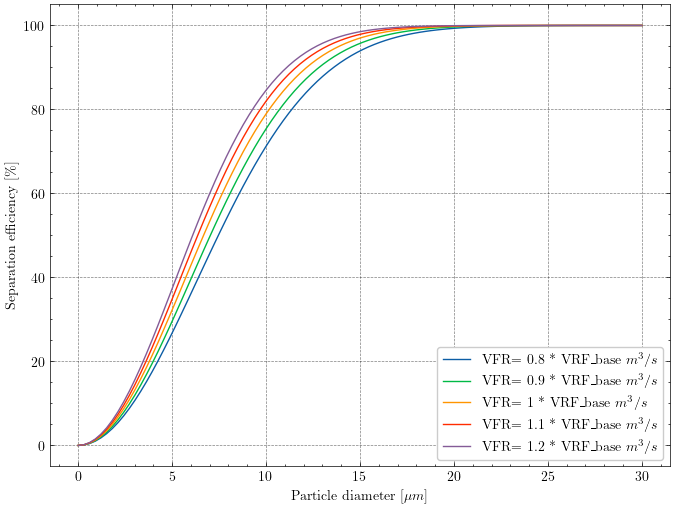
\includegraphics[width=1.0\linewidth]{images/efficiency_vs_inlet_VFR_porcent.png}
		\caption{}
		\label{inlet_VRF_porcent}
	\end{subfigure}
	\begin{subfigure}{.49\textwidth}
		\centering
		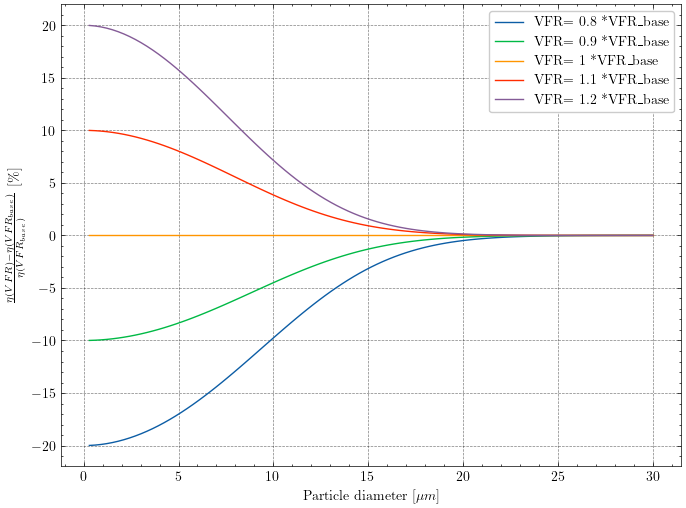
\includegraphics[width=1.0\linewidth]{images/efficiency_vs_inlet_VFR_relative.png}
		\caption{}
		\label{}
	\end{subfigure}
	\captionsetup{font=bf, size=small}
	\caption{ }
	\label{inlet_VRF_relative}
\end{figure}

Figure (\ref{inlet_VRF_relative}) shows  that the efficiency increases proportionally to the increase in VRF when the particle diameter is low. As the diameter of the particle increases, the effect of increasing VRF begins to decrease. However, it must be taken into account that the pressure loss varies with the square of the velocity in the inlet $\left(
\Delta p \propto v_{inlet} ^2 \right)$, so if the flow rate changes 10\% the pressure loss would increase by approximately 21\%.


%EN ALGUN LADO TENGO QUE PONER COMO SE CALCULA LA CONSTANTE KAPPA QUE ESTA RELACIONADA CON EL CAUDAL PARA QUE SE TERMINE DE ENTENDER ESTO.

%VER BIEN ESTA SECCION QUE QUEDO MEDIA FEA


\subsection{Optimization methodology}
In the previous section, the dimensions of a cyclone present in ref.\cite{Zhao2011} were used. That cyclone was used as a reference to see how the efficiency change for some parameters of interest such as temperature or flow rate, but said geometry was not optimal for the problem to be solved. For this reason, in this section the optimization process of the cyclone geometry is presented to maximize the separation efficiency, using both the fluid and the particle materials of interest for the problem.
\subsubsection{Geometrical optimization}

The next section presents how the optimization process was developed. For this, the Python library \texttt{Optimize} is used and \texttt{SLSQP} (Sequential Least Squares Programming) is used as the optimization method. In order to use this method, it is necessary to define the function to be minimized, the variables and both geometric and performance limitations.

In order to define the function, if a  target efficiency $\eta_{target}$ is defined , according to equation (\ref{efficiency_equation}) the radial velocity of the particle is

\begin{equation}
	v_{r,p}= - \frac{ln(1-\eta_{target})}{2 t_{res}} \cdot {R^*} _w
\end{equation}
On the other hand, using the equation (\ref{free_vortex_flow}), (\ref{effective_radious_equation}) and  (\ref{residence_time_equation})  the diameter of the particle can be expressed as:
\begin{align}
	d_p ^2 =&   \frac{18 \mu	v_{r,p}({R^*} _w) {R^*} _w}{\Delta \rho v_{\theta,f} ^2 ({R^*} _w)} \\
	d_p ^2 =&  - \frac{ln(1-\eta_{target})}{2 t_{res}} \cdot \frac{18 \mu {R^*} _w^2}{\Delta \rho v_{\theta,f}^2({R^*} _w) }\\
	d_p ^2 =&  - \frac{ln(1-\eta_{target})}{2 t_{res}} \cdot \frac{18 \mu {R^*} _w^{(2+2n)}}{\kappa^2 }
\end{align}
where the diameter of the particle is defined as a function of the target efficiency, inlet velocity (present in the parameter $\kappa$) and geometry (present in $t_{res}$, ${R^*}_w$ and $\kappa$). With this information, was used as a function to minimize,  the cut diameter defined as  the particle diameter for which the capture efficiency is equal to 50 \% $d_{p,c}=d_p(\eta=50 \%)$:
\begin{equation}
	d_{p.c} (\vec{x})  =  \left(  -  \frac{ln(0.5)}{2 t_{res}} \cdot \frac{18 \mu {R^*} _w^{(2+2n)}}{\kappa^2 }  \right)^{1/2}
\end{equation}

where $\vec{x}=(D,D_e,H,B,h,S,a,b)$ is the vector with all of geometrical variables of the cyclone.

In order to close the problem, the constrains used were:
\begin{enumerate}
	\item $h>S$
	\item $h>a$
	\item $D>D_e+b$
	\item $D_e>b$
	\item $H>S$
	\item $H>h$
	\item $D_e>B$
	\item $10$\textdegree $<\alpha<20$\textdegree , where $\alpha= arctan \left(  \frac{D-B}{2(H-h)} \right) $
	\item $v_{inlet} < v_{max}$
\end{enumerate}

Given that the problem has 8 variables  there are only inequalities as a constrains, more than one local minimum may exist within the domain. For this reason, the optimizer was  initialized with  different seeds in order to obtain the different local minima present in the domain.Then, a family of cyclones was obtained that meet the conditions within the domain, where the cutting diameter varies by less than 10\% and the geometric dimensions change. 



\subsubsection{Optimization: Results}
%(To do : find a better way to calculate the pressure loss throughout the cyclone).
%\begin{equation}
%	Q=\int_{A} v_{\theta,f}(r) dA= a \int_{r_1}^{r_2} \frac{\kappa}{r^n} dr
%\end{equation}
%\begin{equation}
%	\kappa=\frac{Q (1-n)}{a \left(r_2^{(1-n)}-r_1^{(1-n)} \right)}
%\end{equation}
%\begin{equation}
%	v_{\theta,f}(r)=\frac{Q (1-n)}{a  \left(r_2^{(1-n)}-r_1^{(1-n)}  \right)}  \frac{1}{r^n}
%\end{equation}

%Figure () present the the minimum 

%La figura () muestra el valor del diametro de corte en funcion del diametro optimo encontrado usando 256 semillas. se puede observar que a medida que aumenta la cantidad de cyclones en paralelo, el diametro del cyclone disminuye y disminuye considerablemente el diametro de corte. En el caso de utilizar solo un cyclone el diametro necesariamente tiene que ser muy grande para que la velocidad en el inlet no sea demasiado alta. 

%Ademas, la velocidad 

%el cyclone tiene que ser muy chico para poder tener una eficiencia muy alta a 1micro m.con solo un cyclone las dimensiones no son realistas.El cyclone puede servir para poder retirar impuresas de mayor tamano y despues es necesario utilizar algun otro sistema para poder retirar las particulas de menor tamano.

Table (\ref{input_VFR}) show the total volumetric mass flow rate for the commercial and pilot plant calculated in ref. \cite{power_scenario}. 

\begin{table}[H]
	\centering
	\begin{tabular}{ccc}
		\rule[-0.3cm]{0pt}{0.8cm}\textbf{Parameter}               & \textbf{Pilot plant} & \textbf{Commercial plant} \\ \hline
		\rule[-0.3cm]{0pt}{0.8cm}\textbf{VFR per loop {[}m3/s{]}} & 3.27                 & 4.9                       \\ \hline
		\rule[-0.3cm]{0pt}{0.8cm}\textbf{VFR total {[}m3/s{]}}    & 3.27                 & 29.4                     \\ \hline
	\end{tabular}
	\caption{Volumetric flow rate for the pilot and commercial plant calculated in ref. \cite{power_scenario}}
	\label{input_VFR}
\end{table}

For the optimization process, a parametric analysis was carried out where the VFR was varied in the inlet of the cyclone in order to have the same operating conditions in the cyclone for both the commercial and pilot plants and, consequently, the highest separation efficiency with the minimum loss of energy. The ratio between the VFR of the commercial plant and the pilot plant is approximately 9 $\left( \frac{(VFR_{total})_{commercial}}{(VFR_{total})_{pilot}} \approx 9 \right )$ so if you want to have the same efficiency for both plants, it is necessary to increase the number of cyclones 9 times when scaling the plant from the pilot to the commercial one.

%On the other hand, another possible alternative if the maximum number of cyclones for the commercial plant is limited, either due to economic cost or space limitations, etc., figure () shows the sensitivity of the efficiency when varying the VFR inlet in the cyclone. 

Figure (\ref{Fe_d_cut_off}) ,(\ref{Cr_d_cut_off}) and (\ref{AlN_d_cut_off}) shows the cut off diameter ($\eta=50\%$)  for the Fe, Cr and AlN, respectively.  For this analysis, it has been used that the maximum velocity in the inlet has to be less than 25 m/s.

\begin{figure}[H]
	\centering
	\begin{subfigure}{.49\textwidth}
		\centering
		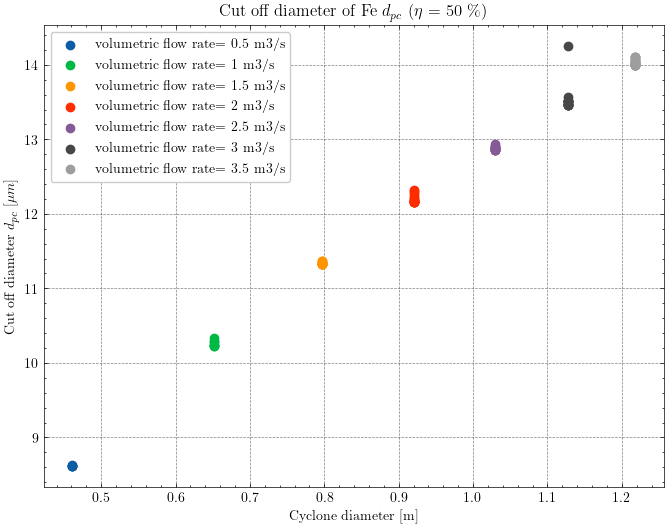
\includegraphics[width=1.0\linewidth]{images/d_pc_Fe.png}
		\caption{}
		\label{Fe_d_cut_off}
	\end{subfigure}
	\begin{subfigure}{.49\textwidth}
		\centering
		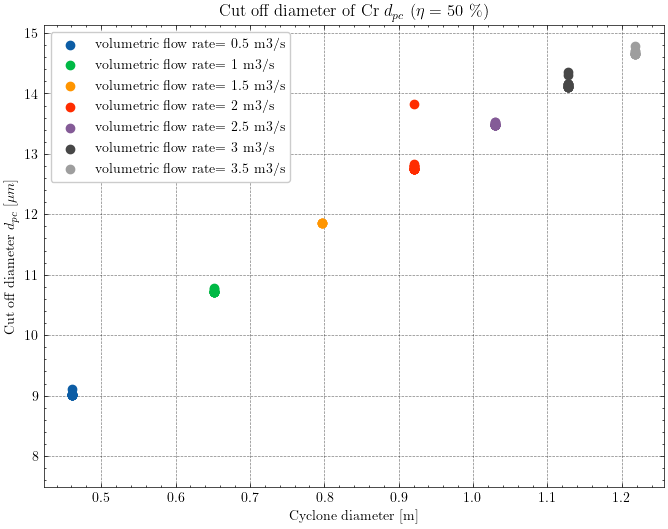
\includegraphics[width=1.0\linewidth]{images/d_pc_Cr.png}
		\caption{}
		\label{Cr_d_cut_off}
	\end{subfigure}
	\begin{subfigure}{.49\textwidth}
		\centering
		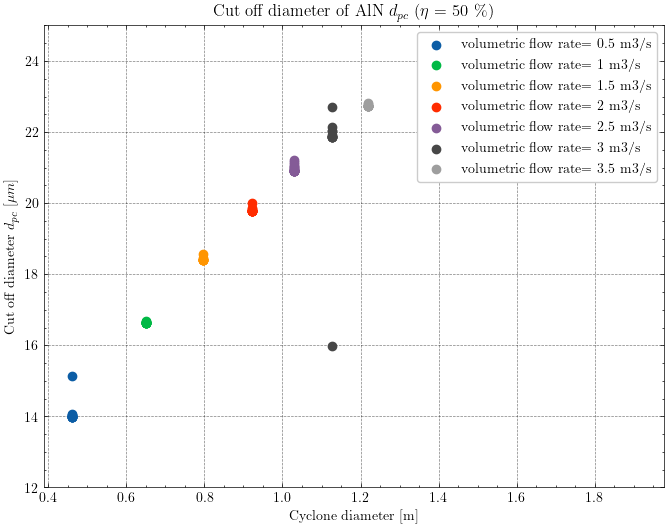
\includegraphics[width=1.0\linewidth]{images/d_pc_AlN.png}
		\caption{}
		\label{AlN_d_cut_off}
	\end{subfigure}
	\captionsetup{font=bf, size=small}
	\caption{ }
	\label{}
\end{figure}

It can be seen that the cutting diameter of both Fe and Cr are quite similar and smaller than that of AlN. This is because the density of Fe is similar to that of Cr, while the density of AlN is much lower. This causes the radial velocity of the particle towards the walls to be lower and the efficiency tends to decrease, so the diameter of the particle must be larger to be captured.

Since the inlet maximum velocity was limited in the optimization process, when the volumetric flow rate increase the cyclone diameter and the inlet dimensions have to grow to have enough space to allocate the inlet and reduce the velocity.    

Table (\ref{info_cyclone}) presents the dimensions of 5 cyclones that can operate at different VFRs. In addition, the cutting diameter for Fe, Cr and AlN is presented and an estimate of the number of cyclones that could be used either in the commercial plant or in the pilot plant.
\begin{table}[H]
	\begin{tabular}{cccccc}
		\rule[-0.3cm]{0pt}{0.8cm}\textbf{Cyclone   case}                                        & \textbf{I} & \textbf{II} & \textbf{III} & \textbf{IV} & \textbf{V} \\ \hline
		\rule[-0.3cm]{0pt}{0.8cm}\textbf{Cyclone body diameter (m)}                             & 0.460      & 0.651       & 0.797        & 0.921       & 1.030      \\\hline
		\rule[-0.3cm]{0pt}{0.8cm}\textbf{Liquid outlet diameter (vortex finder diameter) (m)} & 0.211      & 0.291       & 0.357        & 0.412       & 0.461      \\\hline
		\rule[-0.3cm]{0pt}{0.8cm}\textbf{Cyclone inlet height (m)}                               & 0.230      & 0.326       & 0.399        & 0.460       & 0.515      \\\hline
		\rule[-0.3cm]{0pt}{0.8cm}\textbf{Cyclone inlet width (m)}                          & 0.092      & 0.130       & 0.159        & 0.184       & 0.206      \\\hline
		\rule[-0.3cm]{0pt}{0.8cm}\textbf{Liquid outlet duct length (m)}                         & 0.436      & 0.620       & 0.760        & 0.877       & 0.981      \\\hline
		\rule[-0.3cm]{0pt}{0.8cm}\textbf{Cyclone cylinder height (m)}                           & 1.483      & 2.063       & 2.526        & 2.917       & 3.261      \\\hline
		\rule[-0.3cm]{0pt}{0.8cm}\textbf{Cyclone height (m)}                                    & 0.460      & 0.651       & 0.797        & 0.921       & 1.030      \\\hline
		\rule[-0.3cm]{0pt}{0.8cm}\textbf{Particle outlet diameter (m)}                          & 0.046      & 0.065       & 0.080        & 0.092       & 0.103      \\\hline
		\rule[-0.3cm]{0pt}{0.8cm}\textbf{Angle ($^{\circ}$)}                                                 & 11.453     & 11.723      & 11.732       & 11.731      & 11.731     \\\hline
		\rule[-0.3cm]{0pt}{0.8cm}\textbf{Inlet VFR (m3/s)}                                      & 0.5     & 1.0       & 1.5       & 2.0       & 2.5      \\\hline
		\rule[-0.3cm]{0pt}{0.8cm}\textbf{Inlet Velocity (m/s)}                                        & 23.585     & 23.585      & 23.585       & 23.585      & 23.585     \\\hline
		\rule[-0.3cm]{0pt}{0.8cm}\textbf{Cut off diameter Fe (microns)}                         & 8.610      & 10.230      & 11.322       & 12.053      & 12.864     \\\hline
		\rule[-0.3cm]{0pt}{0.8cm}\textbf{Cut off diameter Cr  (microns)}                        & 9.013      & 10.468      & 11.861       & 12.746      & 13.477     \\\hline
		\rule[-0.3cm]{0pt}{0.8cm}\textbf{Cut off diameter AlN (microns)}                        & 10.207     & 16.620      & 18.393       & 19.765      & 21.215     \\\hline
		\rule[-0.3cm]{0pt}{0.8cm}\textbf{Number of cyclone pilot   plant}                       & 6          & 3           & 2            &             &            \\\hline
		\rule[-0.3cm]{0pt}{0.8cm}\textbf{Number of cyclone commercial plant}                  & 54         & 27          & 18           &             &              \\\hline
	\end{tabular}
	\caption{Cyclone optimization results}
	\label{info_cyclone}
\end{table}


It can be seen that as the volumetric flow rate at the inlet increases, the cut off diameter decrease for all the particles analyzed, causing the lose of separation efficiency. On the other hand, in order to  choose the correct cyclone,the total pressure loss of the system have to be considered. In the literature there are a large number of correlations to calculate pressure loss \cite{Concha2007,Altmeyer2003}, however these are developed mainly for gas-solid cyclones and not for liquid-solid as in this case. For this reason, in the CFD section, importance will be given to the calculation of said parameter.



%\begin{figure}[H]
%	\centering
%	\begin{subfigure}{.49\textwidth}
%		\centering
%		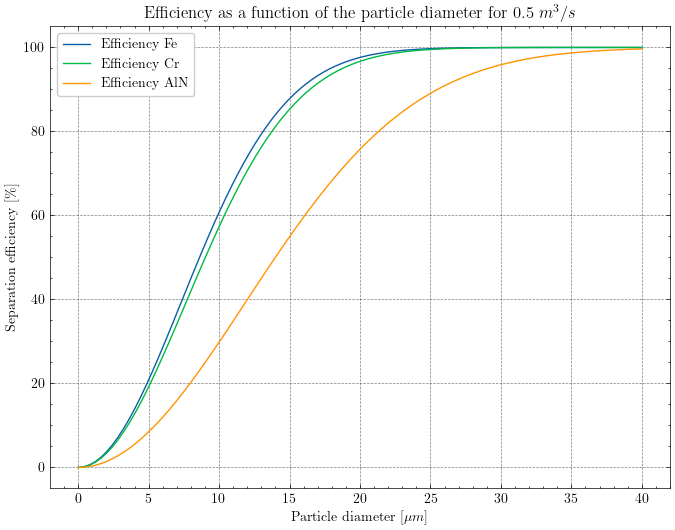
\includegraphics[width=1.0\linewidth]{images/efficiency_for_0.5m3_s.png}
%		\caption{}
%		\label{}
%	\end{subfigure}
%	\begin{subfigure}{.49\textwidth}
%		\centering
%		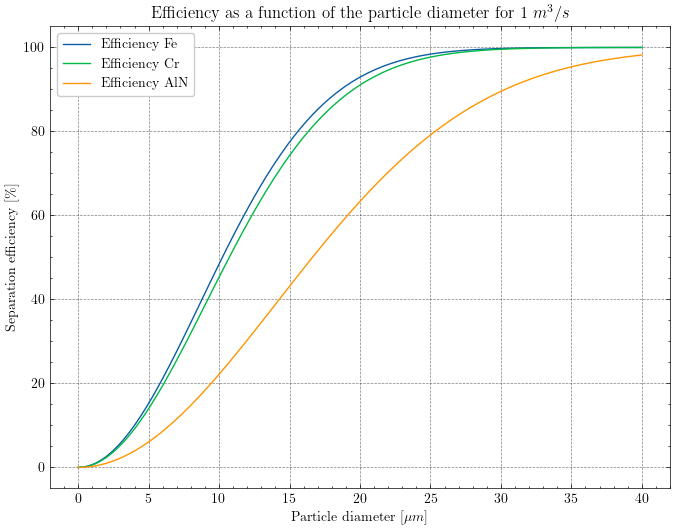
\includegraphics[width=1.0\linewidth]{images/efficiency_for_1m3_s.png}
%		\caption{}
%		\label{}
%	\end{subfigure}
%	\begin{subfigure}{.49\textwidth}
%		\centering
%		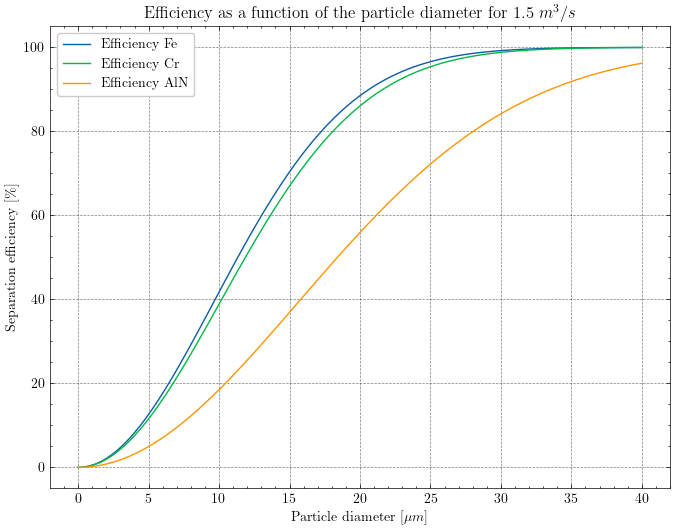
\includegraphics[width=1.0\linewidth]{images/efficiency_for_1.5m3_s.png}
%		\caption{}
%		\label{}
%	\end{subfigure}
%	\captionsetup{font=bf, size=small}
%	\caption{ }
%	\label{}
%\end{figure}





\newpage
\subsection{Conceptual Design Approach}
In the forthcoming project phases, the conceptual design will navigate the design space between the hydrocyclone and Disk Stack Separator, aiming to optimize the multi-stage purification process. With the requirements outlined in Section \ref{sec:sss} and the technical specifications detailed in Figure \ref{multi_stage_technical} serving as foundational guidelines, the design endeavor will seek to exploit the current capabilities of the multi-stage purification system. Drawing inspiration from external sources, such as referenced paper ref. \cite{Van}, the conceptual design will explore innovative approaches (Figure \ref{design_conceptual}) to enhance particle capture efficiency, impurity removal, and overall system performance.\\


\noindent Integration of advanced materials, novel geometries, and optimized operational parameters will be central to the conceptual design exploration. By leveraging insights from existing research and technological advancements, the conceptual design aims to push the boundaries of purification efficiency, ultimately culminating in the development of a device that maximizes the potential of the multi-stage purification process. 


\begin{figure}[H]
	\centering
	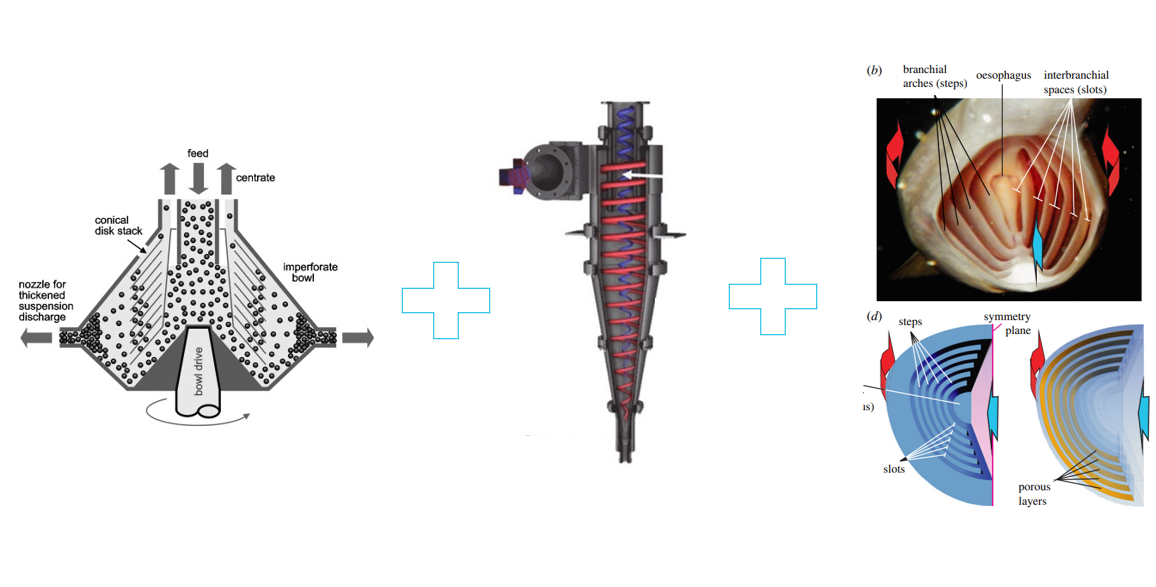
\includegraphics[width=1\linewidth]{design_conceptual.png}
	\captionsetup{font=bf, size=small}
	\caption{Conceptual design approach: possible lines of work}
	\label{design_conceptual}
\end{figure}



\newpage

\section{CONCLUSIONS}








 
xxxxxxxxxxxxxxxxxxxxxxxxxxxxxxxxxxxxxxxxxxxxxxxxxxxxxxxxxxxxxxxxxx





